\documentclass[11pt,a4paper]{article}

\usepackage[utf8]{inputenc}
\usepackage[T1]{fontenc}
\usepackage[french]{babel}
\usepackage{graphicx}
\usepackage{geometry}
\usepackage{float}
\usepackage{hyperref}

\geometry{margin=2cm}
\setlength{\parindent}{0pt}
\setlength{\parskip}{0.6em}

\title{Atelier 1 - Cas d'utilisation d'une station de recharge électrique}
\author{Maxime MANSIET et Simon GODARD}
\date{28 avril 2026}

\begin{document}

\maketitle

\section*{Objectif}
Ce rendu définit le périmètre fonctionnel d'une station de recharge électrique composée d'un hub central et de 4 à 8 bornes. Les diagrammes modélisent les interactions entre les acteurs externes, les services sollicités et la station.

\section{Étape 1 - Services client}
Le diagramme ci-dessous couvre l'expérience du conducteur, inscrit ou anonyme, ainsi que la consultation d'informations publiques par des services numériques tiers.

\begin{figure}[H]
  \centering
  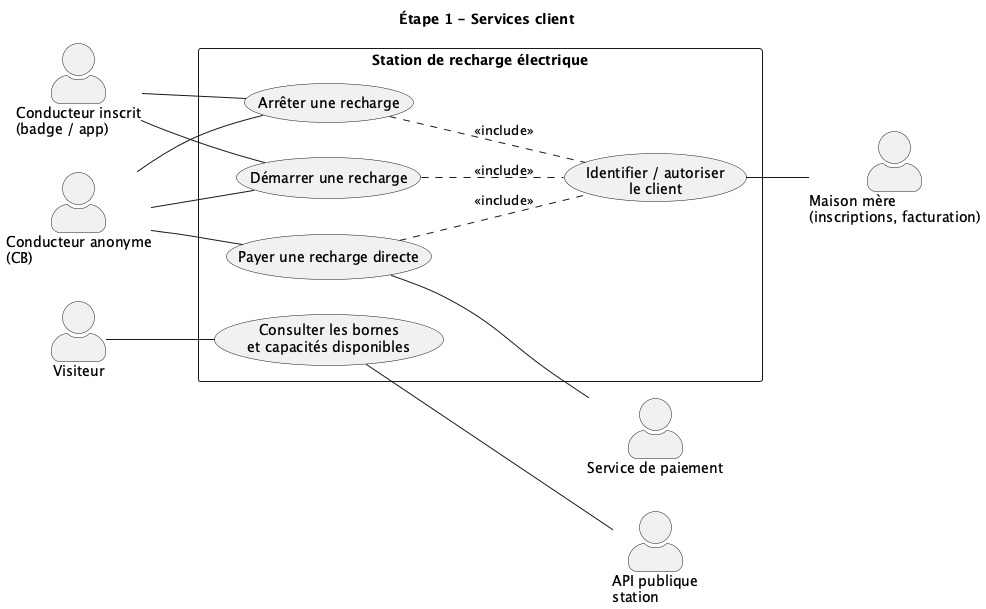
\includegraphics[width=\textwidth,height=0.72\textheight,keepaspectratio]{etape1.png}
  \caption{Services client}
\end{figure}

\section{Étape 2 - Administration et maintenance}
Ce diagramme présente les interactions liées à la mise en service, à la maintenance physique, à la configuration distante, aux tarifs et à la supervision.

\begin{figure}[H]
  \centering
  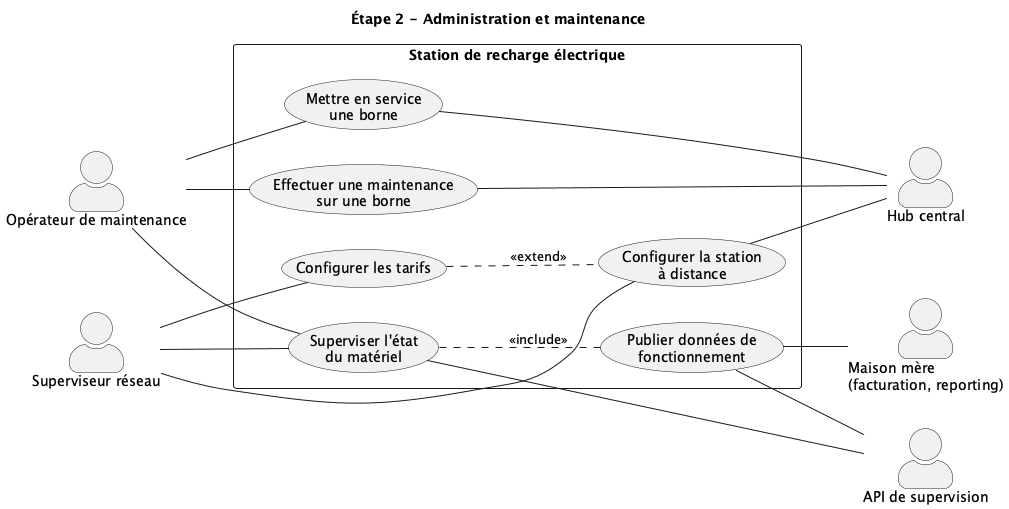
\includegraphics[width=\textwidth,height=0.72\textheight,keepaspectratio]{etape2.png}
  \caption{Administration et maintenance}
\end{figure}

\section{Étape 3 - Délestage}
La contrainte de délestage ajoute le gestionnaire du réseau électrique comme acteur primaire. Celui-ci peut imposer une limitation de puissance à la station, qui répercute ensuite cette contrainte sur la puissance disponible par borne et sur les informations exposées.

\begin{figure}[H]
  \centering
  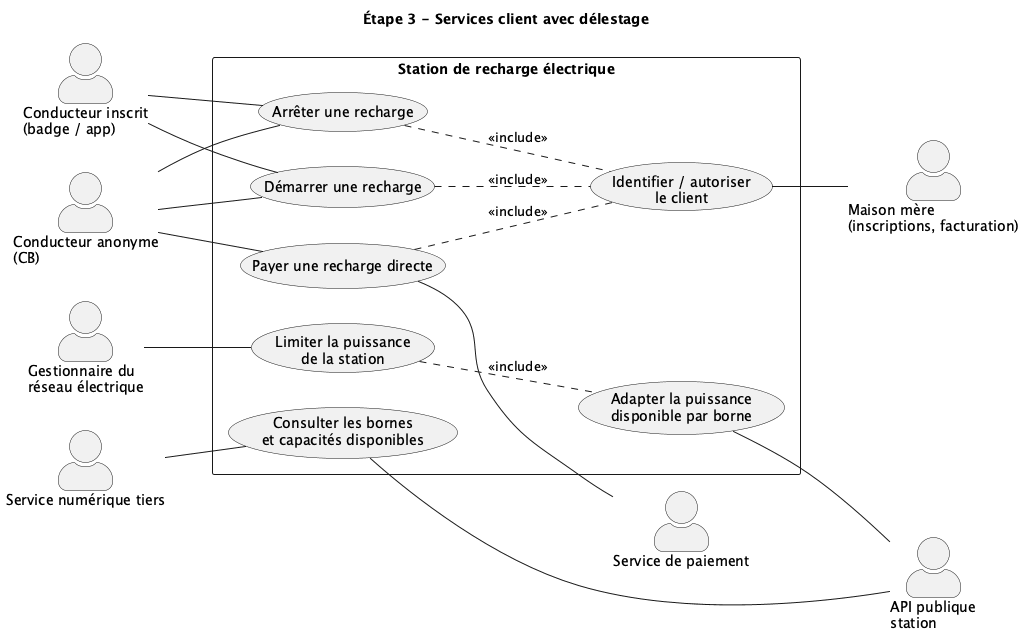
\includegraphics[width=\textwidth,height=0.72\textheight,keepaspectratio]{etape3_clients.png}
  \caption{Services client avec délestage}
\end{figure}

\begin{figure}[H]
  \centering
  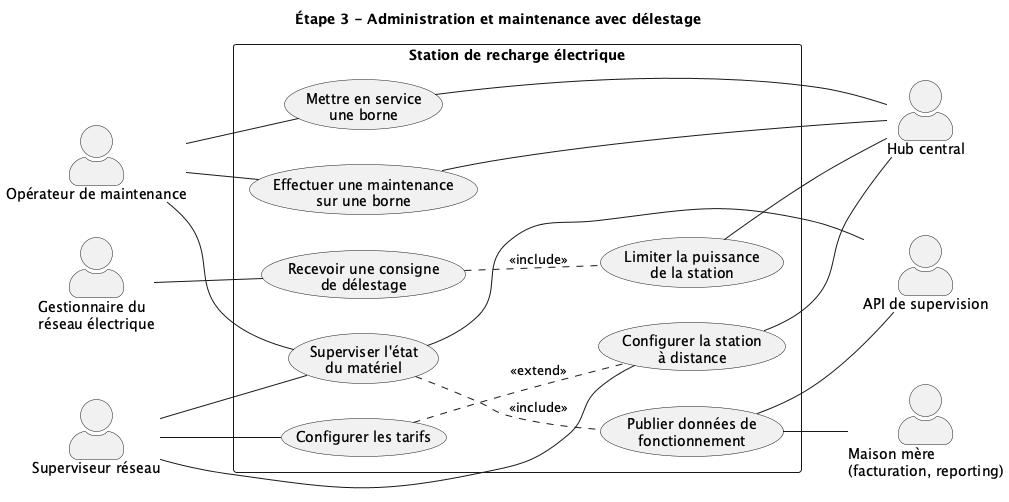
\includegraphics[width=\textwidth,height=0.72\textheight,keepaspectratio]{etape3_admin.png}
  \caption{Administration et maintenance avec délestage}
\end{figure}

\end{document}
